% !TeX root = ../tfg.tex
% !TeX encoding = utf8

\chapter{Quantum Machine Learning}\label{ch:3-QML}


Quantum machine learning is the field that involves the application of machine learning techniques, with the distinctive aspect that quantum computing is integrated at some phase of the process. As seen in \autoref{ch:1-MathematicalFundamentalsML} the basic ingredients of a machine learning setup consists on a computational model to tackle the problem, lots of data to ``feed'' the model and a algorithm of optimization of the configuration of the model so that our model learns from the training data. Therefore, quantum machine learning can vary from the use of a quantum computer in some part of the model, the use of data generated by some quantum process to the use of a quantum computer to process quantum-generated data to achieve improved insights.


In an attempt to further specify the broad world of quantum machine learning we are going to follow the categorization proposed by Schuld and Petruccione in \cite{schuld2021machine}. There are four intersections on the possible ways to combine quantum computing and machine learning depending on the generation of the data (  by a quantum system (Q) or a classical system (C)) and the information processing device (being a quantum (Q) or a classical (C) device).
\begin{itemize}
    \item The CC intersection covers classical data being processed classically, which is the conventional approach to machine learning, but in this contexts, it concerns the classical machine learning techniques that are based on ideas from quantum computing. So there is no actual quantum computing involved in this approach, just some inspiration.
    \item The QC intersection considers classical machine learning algorithms that operate on quantum data. It can be understood whether as classical machine learning methods that are run on data generated by quantum processes or as the application of classical machine learning to quantum computing. 
    \item The kind of quantum machine learning that is referred on this thesis and in the bibliography taken into consideration is the intersection CQ: classical data being processed by a quantum computer. These machine learning techniques are implemented within a quantum computer that is fed classical data. Quantum computing is involved in the model or in the training of the machine learning techniques.
    \item Ultimately, there is the QQ category that works on quantum data being processed by a quantum computer. As in the CQ intersection, quantum computing may be involved in the models or in the training processes, but in this case, the quantum data needs to come from measuring a quantum system (in a physical experiment or in a simulation of it run on a quantum computer) such as \cite{Perrier_QDataSet_Quantum_Datasets_2021} and \cite{schatzki2021entangled} proposals. QQ can be viewed as an extension of CQ and it is definitely a promising area but the required technologies and research on this intersection are still scarce.
\end{itemize}

\begin{figure}
    \centering
    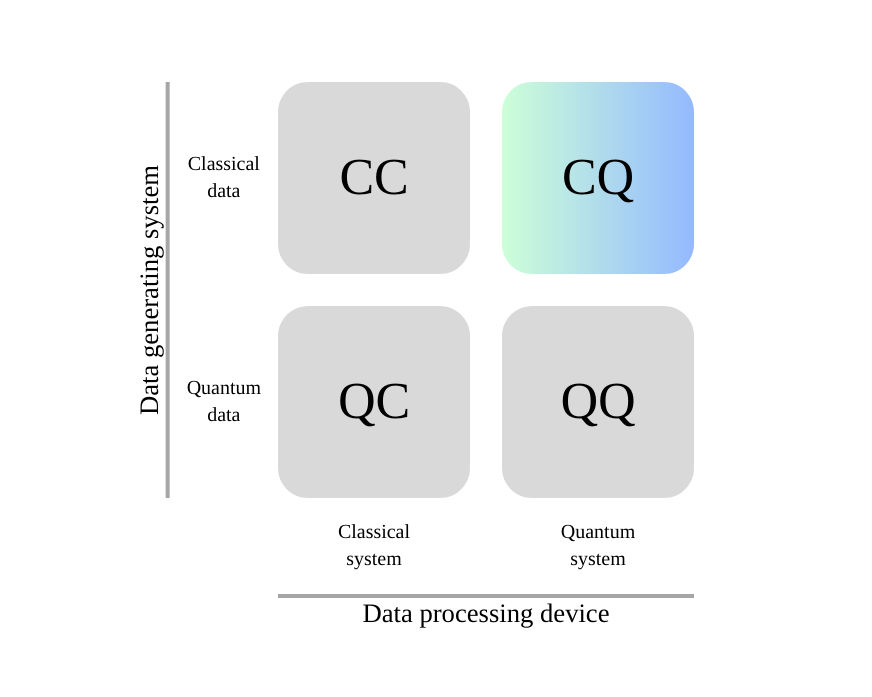
\includegraphics[width=\linewidth]{img/img-ch3/four_intersections_ML-QC.png}
    \caption{The four approaches to combine quantum computing and machine learning, categorized according to the nature of the data and the system used}
    \label{fig:four-intersections}
\end{figure}

In this thesis we will focus on CQ quantum machine learning, but within this category there is a broad range of possibilities. We will leave aside the proposals of  quantum algorithms that could speed up classical machine learning because they rely on a full error-corrected quantum computer that is currently beyond the limits of the state-of-the-art. Instead, we will dedicate to the study of fully quantum-oriented models that can be run on NISQ devices. \footnote{NISQ stands for noise intermediate-scale quantum computers, that are at our disposal now.} The goal is to use a quantum device as a machine learning model, not just as an alternative hardware to accelerate computation. This leads to new models and training algorithms derived from a quantum computational paradigm that require a the solid understanding of the intricacies of machine learning. Exploring the possibilities of NISQ computers and machine learning algorithms suitable to be executed on them will be a crucial field in the short and medium terms. It may bring us closer to the way for the first practical applications of quantum computing come to life. 

\section{Quantum support vector machines} \label{sec:QSVM}
Quantum support vector machines are a particular case of general support vector machines that rely on kernel methods in which we use quantum computers to map data into a space of quantum states. The kernel method, as seen in \autoref{subs:kernel-methods}, consists in mapping the data from its original space to a higher dimensional space known as feature space in which we wish our data could be separable by a hyperplane. In other words, by raising the dimensionality, the so called feature map can transform the problem into a linearly separable one. Quantum computing and kernel methods are based on a similar principle, a straightforward way to visualize it is presented in \autoref{fig:parallelism}. Both have mathematical frameworks in which information is mapped into and then processed in high-dimensional spaces to which we have only limited access. In kernel methods, the access to the feature space is facilitated though kernels (which are inner products of feature vectors). In quantum computing, access to the Hilbert space of quantum states is given by measurements, which can also be expressed through inner products of quantum states.

\begin{figure}
    \centering
    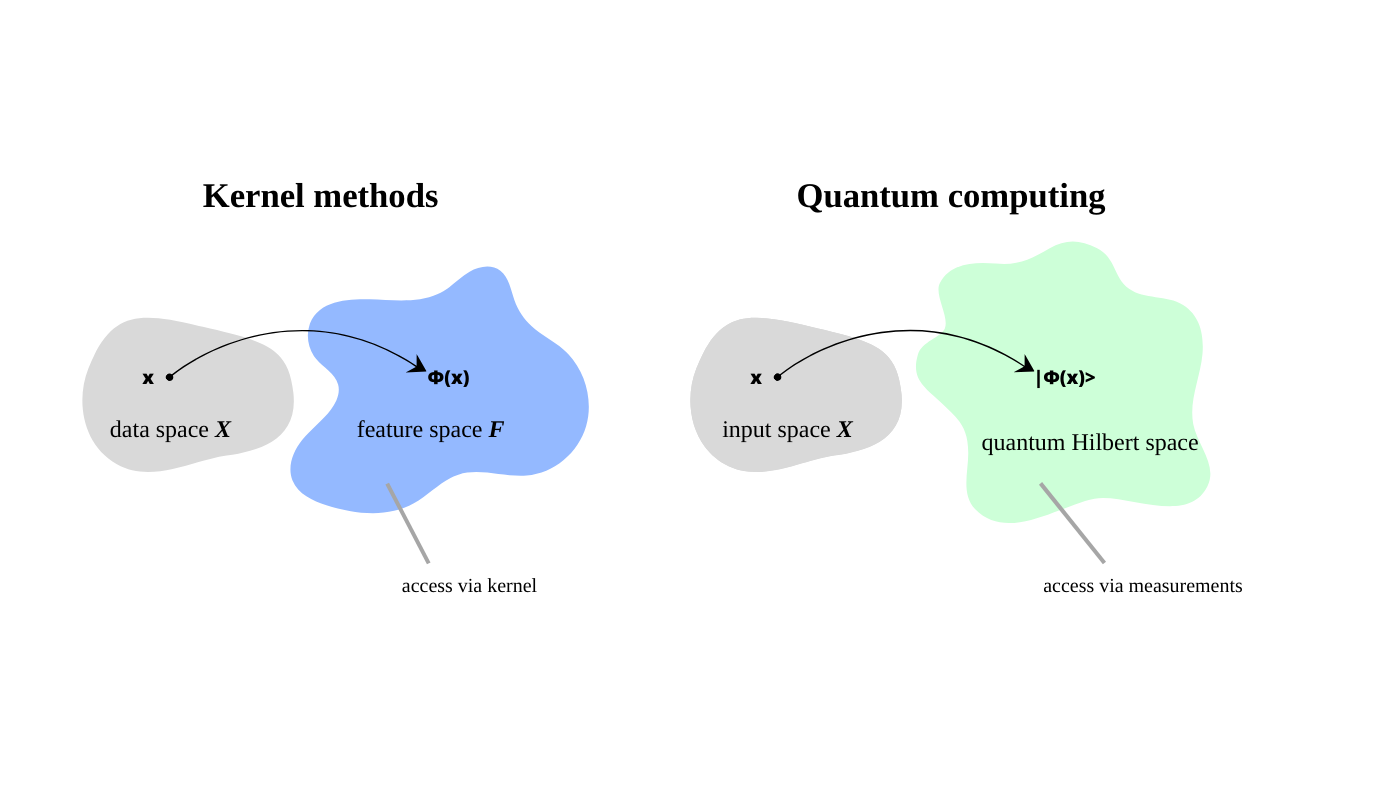
\includegraphics[width=\linewidth]{img/img-ch3/paralelism_KM-QC.png}
    \caption{Parallelism between the framework of kernel methods and the world of quantum computing. Illustration of own production inspired by \cite{schuld2021machine}.}
    \label{fig:parallelism}
\end{figure}


Therefore, we can view quantum support vector machine as ordinary support vector machines that rely on kernel methods where the feature space $\mathcal{F}$ is a certain space of quantum states. In order to train and use QSVM for classification, we will be able to operate as usual with classical SVM, except for the computation of the kernel function, which will require a quantum computer to
\begin{enumerate}
    \item Take as input two vectors in the original space of data, $\mathcal{X}$.
    \item Map each vector to a quantum state through a feature map, $\Phi$.
    \item Compute the inner product of the  quantum states and return it.
\end{enumerate}

Let's dive deeper into the mathematical framework that supports QSVM.
Kernel theory in feature space for machine learning uses linear algebra and functional analysis as tools to  pull data to a feature space for the sake of better discrimination of classes or simpler representation of data. 

\subsection{Feature map}\label{subsec: feature map}
Feature maps play an important role in machine learning, since they map any type of input data into a higher dimensional space with a well-defined metric. 

Essentially feature maps are just circuits that are parametrized exclusively by the original (classical) data and thus prepare a quantum state that depends only on that data. Consider a data embedding circuit $\Phi$ that depends on some classical data $x \in \mathcal{X}$. For each input $x \in \mathcal{X}$, we will have a circuit $\Phi(x)$ such that the output of the feature map will be the quantum state $\varphi(x)=\Phi(x) \ket 0$. 

%\textcolor{blue}{From the quantum physics perspective $x \longrightarrow \ket{\varphi(x)}$ would be a valid feature map, nevertheless it's not a good choice of feature map to then be able to apply comfortably the kernel theory since \textbf{quantum models are not linear in the Hilbert space of the quantum system}\footnote{ WHY? I can't really see why}. Instead the quantum feature map of choice will be $x \longrightarrow \phi(x) = \ket{\varphi(x)} \bra{\varphi(x)}$.}

\begin{definicion}[Feature map]
    Given a Hilbert space $\mathcal{F}$, called the feature space, an input set $\mathcal{X}$ and $x \in \mathcal{X}$ a sample from the input set. A feature map is a map $\Phi : \mathcal{X \longrightarrow \mathcal{F}}$ from inputs to vectors in the Hilbert space. The vectors $\Phi(x) \in \mathcal{F}$ are called feature vectors.      
\end{definicion}

By definition of inner product, every feature map gives rise to a kernel.

\begin{teorema}\label{th:feature map->kernel}
    Given a feature map $\Phi: \mathcal{X} \longrightarrow \mathcal{F}$. The inner product defined in the feature space of two feature vectors (obtained via the feature map) defines a kernel. 
    $$\kappa(x,y)=\left< \Phi(x), \Phi(y) \right>_{\mathcal{F}}$$
\end{teorema}
\begin{proof}
    We shall see that the previously defined kernel is a semi-definite function by showing that its Gram matrix is positive definite. 
    Let $c_i,c_j \in \mathbb{C}$ and $x_i \in \mathcal{X}$ for $i,j \subseteq \left\lbrace1,...M\right\rbrace$ with $M \geq 2$
    \begin{equation*}
        \sum_{i,j=1}^M c_i c_j \kappa(x_i,x_j) = \left< \sum_{i=1}^M c_i \Phi(x_i) , \sum_{j=1}^M c_j \Phi(x_j) \right> = ||\sum_{i=1}^M c_i \Phi(x_i) ||^2 \geq 0 
    \end{equation*}
\end{proof}


\subsection{Reproducing kernel Hilbert spaces}
Kernel theory gives rise to the reproducing kernel Hilbert space (RKHS), a rather abstract concept yet useful in order to understand the importance of kernels for machine learning, as their connection to linear models in feature space. 

So far, we are dealing with two Hilbert spaces: the Hilbert space of the quantum system and the feature space $\mathcal{F}$ that contains the embedded data by the feature map. Now we will build another feature space for the quantum kernel, derived directly from the kernel. This feature space is a Hilbert space $\mathcal{R}$ of functions and due to its definition it is called the reproducing kernel Hilbert space.

\begin{definicion}[RKHS]
    Let $\mathcal{X}$ be a non-empty input set and $\mathcal{R}$ a Hilbert space of functions $f:\mathcal{X} \longrightarrow \mathbb{K}$ that map inputs to real numbers. Let $\left< \cdot, \cdot \right>$ be the inner product on $\mathcal{R}$. \\$\mathcal{R}$ is a reproducing kernel Hilbert space if every point evaluation is a continuous functional $ F: f \longrightarrow f(x) \quad \forall x \in \mathcal{X}$. This condition is equivalent to the condition that there exists a function $\kappa : \mathcal{X} \times \mathcal{X} \longrightarrow \mathbb{K}$ for which $\left< f, \kappa(x,\cdot)\right> = f(x)$, with $\kappa(x,\cdot) \in \mathcal{R}, \forall f \in \mathcal{H}, x \in \mathcal{X}$. 
    
    The function $\kappa$ is the unique reproducing kernel of $\mathcal{R}$. 
    
    % A Reproducing Kernel Hilbert Space (RKHS) is a Hilbert space $\mathcal{H}$ of functions $f:\mathcal{X} \longrightarrow \mathbb{K}$ with a reproducing kernel $\kappa : \mathcal{X} \times \mathcal{X}  \longrightarrow \mathbb{K}$ where $\kappa(x,\cdot)\in \mathcal{H}$ and $f(x)=\left< \kappa(x,y), f \right> \quad \forall y \in \mathcal{X}$.
\end{definicion}

To understand it better let's consider a kernel function of two variables $\kappa(x,y)$. For $n$ points we fix one of the variables to have $\kappa(x_1,y)$, $\kappa(x_2,y)$,..., $\kappa(x_n,y)$. These are $n$ functions of the variable $y$. RKHS is a function space which is the set of all possible linear combinations of these functions:
\begin{equation}
    \mathcal{R} = \left\lbrace f(\cdot)=\sum_{i=1}^{n} \alpha \kappa(x_i, \cdot) \quad \forall y \in \mathcal{X} \right\rbrace
\end{equation}

As we have just seen, the functions that belong to the RKHS are linear combinations of its elementary kernel functions $\kappa(x,\cdot)$ where one variable is fixed in a possible data sample $x \in \mathcal{X}$. This kernel $\kappa(x,\cdot)$ assign a distance measure to every data point. Computing $\kappa(x,y)$ gives us the distance between the two points $x,y \in \mathcal{X}$. 
Therefore, the functions $ f(y)=\sum_{i=1}^{n} \alpha \kappa(x_i, y) \in \mathcal{R}$ are linear combinations of data similarities. 

For example, using one of the most widely used kernels, a Gaussian kernel $$\kappa(x,y)=\exp{\frac{|| x-y || }{2 \sigma^2}}$$ the functions $f \in \mathcal{R}$ are linear combinations of Gaussians centred in each data point. The kernel regulates the ``smoothness'' of the functions in $\mathcal{R}$ by changing the variance of the Gaussian. 

In order to calculate the inner product of two functions in RKHS $f, g \in \mathcal{R}$, since every function in RKHS can be written as a linear combination, $f=\sum_{i=1}^n \alpha_i \kappa(x_i, \cdot)$ and $g= \sum_{j=1}^n \beta_j \kappa(y_j, \cdot)$, 
\begin{align}\label{eq:inner-product-RKHS}
    \left< f, g\right> 
    &= \left< \sum_{i=1}^n \alpha_i \kappa(x_i,\cdot), \sum_{j=1}^n \beta_j \kappa(y_j, \cdot) \right> \\
    &\stackrel{(1)}{=}  \left< \sum_{i=1}^n \alpha_i \kappa(x_i,\cdot), \sum_{j=1}^n \beta_j \kappa(\cdot, y_j) \right> \\
    &= \sum_{i=1}^n \sum_{j=1}^n \alpha_i \beta_j \kappa(x_i, y_j)  
\end{align}

where $(1)$ uses that the kernel is symmetric. 
Indeed this is a well-defined inner product:
\begin{enumerate}
    \item It is symmetric, because so it is $\kappa$
    $$\left<g,f\right>= \sum_{j=1}^n \sum_{i=1}^n \beta_j \alpha_i \kappa(y_j, x_i) = \left<f,g\right>$$
    \item It is bilinear

    Observe,
    $$\left<f,g \right>= \sum_{j=1}^n \beta_j \sum_{i=1}^n \alpha_i \kappa(x_i, y_j) = \sum_{j=1}^n \beta_j f(y_j) $$

    Then we have,
    \begin{align}
        \left< f_1 + f_2, g\right> &= \sum_{j=1}^n \beta_j (f_1(y_j) + f_2(y_j)) \\
        &= \sum_{j=1}^n \beta_j f_1(y_j) + \sum_{j=1}^n \beta_j f_2(y_j) \\
        &= \left< f_1, g \right> + \left< f_2, g\right>
    \end{align}

    Similarly, we can show that $\left<f, g_1 + g_2 \right> = \left< f,g_1\right> + \left< f,g_2 \right>$
    \item It is positive semi-definite, since the kernel $\kappa$ is positive semi-definite. Next we will see that in fact, it is strictly positive definite. It is the last characteristic missing to prove it is an valid inner product.
\end{enumerate}

The name RKHS consists on several parts, let's analyse its meaning:
\begin{itemize}
    \item ``Reproducing'' because of the reproducing property of this space.
    
    We consider $g \in \mathcal{R}$ a kernel in RKHS space. In other words, we take $g$ to have only one component ${g(x)=\sum_{j=1}^n \beta_j \kappa(x_i,x) = \beta \kappa(x,x)}$. We take $\beta=1$ to have $g(x)=\kappa (x,x) $. 
    
    We also consider $f \in \mathcal{R}$ as  $f=\sum_{i=1}^n \alpha_i \kappa(x_i,y)$. According to \autoref{eq:inner-product-RKHS}, the inner product of $f,g \in \mathcal{R}$ is:
    \begin{align}
        \left< f(x), g(x)\right> &= \left< f, \kappa_x(\cdot) \right> \\
        &= \left< \sum_{i=1}^n \alpha_i \kappa(x_i,x) , \kappa (x,x) \right> \\
        &= \sum_{i=1}^n \alpha_i \kappa(x_i,x) = f(x)
    \end{align}
    This means that the function f is reproduced from the inner product of that function with one of the kernels of the space. In conclusion, the reproducing property is $$\left< f, \kappa(x,\cdot)\right> = f(x) $$ with $\kappa(x,\cdot), f \in \mathcal{R}, x \in \mathcal{X}$. 

    It is worth pointing out the special case
    \begin{equation*}\label{eq:special case reproducing property}
        \left< \kappa(x, \cdot), \kappa(x, \cdot) \right> = \kappa(x,x)
    \end{equation*}
    
    \item ``Kernel'' because of the kernels associated to RKHS as priorly stated.
    
    \item ``Hilbert space'': because $\mathcal{R}$ is a complete prehilbertian space. 
    
    We need to check that $\left<\cdot, \cdot\right>$ is strictly positive definite:
    \begin{equation*}
        |f(x)|^2 \stackrel{(1)}{=} |\left< \kappa(x, \cdot), f\right>|^2 \stackrel{(2)}{\leq} \left< \kappa(x, \cdot), \kappa(x, \cdot) \right> \cdot \left< f, f \right> = \kappa(x,x) \left<f, f \right>
    \end{equation*}
    where we use
    \begin{enumerate}
        \item The reproducing property
        \item The special case of the reproducing property \autoref{eq:special case reproducing property}
    \end{enumerate}
    It follows that $\left<f,f\right> = 0$ if $f=0$ is the identically null function. Therefore $\left<\cdot ,\cdot \right>$ is strictly positive definite and we can claim that it is an inner product.
    Now, we consider the norm $$||f|| = \sqrt{\left<f,f\right>}$$ $\mathcal{R}$ includes the limit points of sequences that converge in that norm. That makes it a complete space.
\end{itemize}


Since a feature map induces a kernel and a kernel gives rise to a reproducing kernel Hilbert space, we can construct a unique reproducing kernel Hilbert space for any given feature map.

\begin{teorema}\label{th:kernel->RKHS}
    Let $\Phi:\mathcal{X} \longrightarrow \mathcal{F}$ be a feature map over an input set $\mathcal{X}$, giving rise to a complex kernel $\kappa(x,y)=\left<\Phi(x),\Phi(y) \right>_{\mathcal{F}}$. The corresponding reproducing kernel Hilbert space has the form 
    \begin{equation} \label{eq:Rk}
        \mathcal{R}_{\kappa} = \left\lbrace f: \mathcal{X} \longrightarrow \mathbb{K} \,|\, f(x) = \left< w, \Phi(x) \right>_{\mathcal{F}}, \quad \forall x\in \mathcal{X}, w \in \mathcal{F} \right\rbrace
    \end{equation}
\end{teorema}

\begin{definicion}[Linear models]
    Let $\mathcal{X}$ be a data domain and $\Phi: \mathcal{X} \longrightarrow \mathcal{F}$ a feature map. A linear model in $\mathcal{F}$ is a function that maps every $x \in \mathcal{X}$ to the inner product of its feature map $\Phi(x)$ and a certain vector in the feature space $w \in \mathcal{F}$. Formally,
    $$f(x) = \left< \Phi(x), w \right>_{\mathcal{F}}$$ with $w \in \mathcal{F}$.
\end{definicion}

\begin{teorema}
    Deterministic quantum models are linear models in data-encoding feature space. Let $f(x)=\mathrm{tr} \left\lbrace \rho \mathcal{M} \right\rbrace$ be a quantum model and $\Phi: \mathcal{X} \longrightarrow \mathcal{F}$ the feature map $\Phi(x)=\rho(x) \in \mathcal{F}$. The quantum model $f$ is a linear model in $\mathcal{F}$.
\end{teorema}

This was the missing point to understand the relevance of the reproducing kernel Hilbert space: the functions living in the RKHS are the quantum model functions, which we have just stated that are linear models. Thus, the RKHS is equivalent to the space of linear models derived from the reproducing kernel. To conclude, the kernel essentially defines the class of functions that the linear model can express and, as a result, learn.

As seen in \autoref{eq:Rk}, the functions $\left< w, \cdot \right>$ in the RKHS $\mathcal{R}_{\kappa}$  associated with feature map $\Phi$ can be interpreted as linear models for which $w \in \mathcal{F}$ defines a hyperplane in feature space. 

%\textcolor{green}{Include theorems 6.3 and 6.4 from \cite{schuld2021machine}?}

\subsection{Quantum kernels}

As anticipated in \autoref{subs:kernel-methods}, the relation between kernels and inner products has a great importance in machine learning since they are a means of computation in the feature space without having to deal with the feature vectors $\Phi(x)$. Therefore, the classifier can be inferred from a kernel function that encodes the scalar product between the new features.

Now, let the feature space be the Hilbert space of the quantum system. We want to find out the kernel associated to that system, which we will call the quantum kernel. The methodology of work would be to encode some input $x \in  \mathcal{X}$ into a quantum state $\ket{\Phi(x)} \in \mathcal{F}$ described by a vector in the feature Hilbert space. This ``input-encoding'' procedure corresponds to what we have defined as \textbf{feature map} $\Phi: \mathcal{X} \longrightarrow \mathcal{F}$. There are different input encoding techniques in quantum machine learning, we discuss more on them in this section. According to \autoref{th:feature map->kernel} the feature map $\Phi$ induces a kernel $\kappa$:
$$ \kappa(x,y)=\left< \Phi(x), \Phi(y) \right>_{\mathcal{F}} \quad \forall x,y \in \mathcal{X}$$
As stated by \autoref{th:kernel->RKHS} the kernel $\kappa$ induces a RKHS $\mathcal{R}_{\kappa}$ (where $\kappa$ is the reproducing kernel). The functions in $\mathcal{R}_{\kappa}$ are the inner products of the feature maps of the input data and a vector $\ket{w} \in \mathcal{F}$ which defines a linear model $$ f(x, w) = \braket{w | \Phi(x)} $$
Note that we use Dirac brackets $\braket{\cdot | \cdot}$ instead of the inner product $\left< \cdot , \cdot \right>$ to denote the inner produts in a quantum Hilbert space.

It is worth pointing out that the idea of interpreting $ x \longrightarrow \ket{\Phi(x)}$ is the starting point that allows us to make use of the entire framework of kernel theory. 

\begin{definicion}[Quantum kernel]
    Given $\Phi$ a feature map over an input domain $\mathcal{X}$. A quantum kernel is the Hilbert-Schmidt inner product between two feature vectors $\varphi(x), \varphi(y)$ where $x,y \in \mathcal{X}$:
    \begin{equation}
        \kappa(x,y) = \mathrm{tr} \left\lbrace \varphi(y), \varphi(x) \right\rbrace = |\braket{\Phi(y)|\Phi(x)}|^2
    \end{equation}
\end{definicion}


The quantum kernel previously defined is indeed a kernel because it is a positive definite function. We can see that it is a product of the complex kernel $\kappa(x,y) = \braket{\Phi(y)|\Phi(x)}$ and its complex conjugate $\kappa(x,y)^*=\braket{\Phi(x)|\Phi(y)}$. It is needed to check that the complex conjugate of a kernel is a kernel itself. Given $x_i \in \mathcal{X}, \quad i=1,...,n$ and $c_i \in \mathbf{C}$,
\begin{align}
    \sum_{i,j=1}^n c_i c_j^*(\kappa(x_i,x_j))^* &= \sum_{i,j=1} c_i c_j^* \left< \Phi(x_i), \Phi(x_j)\right> \\
    &= (\sum_{i=1}^n c_i \bra{\Phi(x_i)}) \cdot (\sum_{i=1}^n c_i^* \ket{\Phi(x_i)}) \\
    &= || \sum_{i=1}^n c_i^* \ket{\Phi(x_i)} ||^2 \geq 0
\end{align}
So the complex conjugate of a kernel is also positive definite.

Lastly, the product of two kernels is known to be a kernel.


To bring to life the definition of quantum kernel, we need to dive into different examples of data encoding feature maps, its feature-embedding circuits and kernels they give rise to.

\begin{enumerate}
    \item \textbf{Basis encoding.} The data encoding feature map of basis encoding maps a $n$ bit binary string $x = (b_1,...b_n) $ with $b_i \in \left\lbrace 0,1\right\rbrace, \quad i=1,...,n$ to a computational basis state in a $n$-qubit system, which in turn corresponds to a standard basis vector $ \ket{i_x}$ , with $i_x$ being the integer representation of the bitstring), in a $2^n$-dimensional Hilbert feature space. This feature map is given by $$\Phi: x \in \left\lbrace 0,1 \right\rbrace^n \longrightarrow \ket{i_x} $$

    Basically this feature map maps each data input to a state from an orthonormal basis.

    The associated quantum kernel is the Kronecker delta
    $$\kappa(x,y) = \left< \Phi(x), \Phi(y) \right>_{\mathcal{F}} = \braket{i_x|i_y} \stackrel{(1)}{=} \delta_{x,y}$$

    in $(1)$ we observe we are computing the inner product in a quantum Hilbert space (hence the Dirac notation)  of orthonormal states by definition of the feature map. 
    
    This kernel is a binary similarity measure on the input space that is only nonzero for two identical inputs, thus really strict and hardly ever a good choice of data encoding for quantum machine learning tasks.
    
    \item \textbf{Amplitude encoding. } The data encoding feature map of amplitude encoding maps each input vector into the amplitudes of a quantum state with respect to a fixed basis, the orthonormal computational basis. Let $\mathbf{x}=(x_0,...,x_{N-1} ) \in \mathbb{R}^N $ be a input vector of dimension $N=2^n$. This encoding technique maps it to the amplitudes of a $n$-qubit state $\ket{\psi_{\mathbf{x}}}$.
    \begin{equation*}
        \Phi: \mathbf{x}\in \mathbb{R}^N \longrightarrow \ket{\psi_{\mathbf{x}}} = \frac{1}{\sqrt{\sum_{i}x_i^2}} \sum_{i=0}^{N-1} x_i \ket{i}
    \end{equation*}

    where $\ket{i}$ denotes the i-th computational basis state. 
    It is worth pointing out that we have included a normalization factor to make sure that the output is, indeed, a quantum state. This definition of amplitude encoding doesn't work for the null vector.
    
    Amplitude encoding offers an important benefit in terms of spatial efficiency compared to basis encoding. Using basis encoding, in a $n$-qubit system we can only codify strings of $n$ classical bits, whereas using amplitude encoding we can store vectors of dimension $2^n$. 

    The associated quantum kernel is:
    $$\kappa(\mathbf{x},\mathrm{y})=\left< \Phi(\mathbf{x}),\Phi(\mathrm{y}) \right> = \braket{\psi_{\mathbf{x}} | \psi_{\mathrm{y}}} = \mathbf{x}^{T} \mathrm{y}$$

    \item \textbf{Copies of quantum states. } Similarly done as in amplitude encoding, this data encoding technique maps each input vector $\mathbf{x} \in \mathbb{R}^N$ to $d$ copies of an amplitude encoded quantum state.
    \begin{equation*}
        \Phi: \mathbf{x}\in \mathbb{R}^N \longrightarrow \ket{\psi_{\mathbf{x}}} \otimes ... \otimes \ket{\psi_{\mathbf{x}}}
    \end{equation*}
    The associated quantum kernel is known as homogeneus polynomial kernel
    $$\kappa(\mathbf{x},\mathrm{y})=\left< \Phi(\mathbf{x}),\Phi(\mathrm{y}) \right> = \braket{\psi_{\mathbf{x}} | \psi_{\mathrm{y}}} \otimes ... \otimes \braket{\psi_{\mathbf{x}} | \psi_{\mathrm{y}}} = (\mathbf{x}^{T} \mathrm{y})^d$$

\end{enumerate}


% From practical book Finally we observe that it is equivalent to computing the probability of measuring all zeros after preparing the state $\Phi^*(x) \Phi(y) \ket{0}$. Therefore, the kernel operation results to be 
%\begin{equation}
 %   \kappa(x,y) = |\braket{0| \Phi^*(x) \Phi(y) | 0} |^2
%\end{equation}

% From practical book To sum up, the implementation of a quantum kernel function consists on taking a feature map that returns a circuit $\Phi(x)$ for any input $x \in \mathcal{X}$, then preparing the state $\Phi^*(x) \Phi(y) \ket{0}$ for the pair of vector $x,y$ on which we want to compute the kernel and finally returning the probability of measuring zero on all the qubits.


Next, we will go through one of the main achievements of classical kernel theory: the representer theorem. It states that the function $f$ from the RKHS which minimises the cost function can always be expressed as a weighted sum of the kernel between $x$ and the training data. 

\begin{teorema}[Representer theorem]
    Given $\mathcal{X}$ an input domain, $\mathcal{Y}$ an output domain. Let $\kappa$ be $\kappa: \mathcal{X} \times \mathcal{Y} \longrightarrow \mathbb{R}$ a kernel, with a corresponding reproducing kernel Hilbert space $\mathcal{R}_{\kappa}$, $\mathcal{D}$ a training data set consisting of $M$ data pairs $\mathcal{D} = \left\lbrace (x_1,y_1),...,(x_M,y_M) \in \mathcal{X} \times \mathcal{Y} \right\rbrace$. Assume a cost function $C$ that quantifies the quality of a model by comparing predicted outputs $f(x_i)$ with targets $y_i$ and consider a strictly monotonic increasing regularisation function $g: \interval[open right]{0}{\infty} \longrightarrow \mathbb{R}$.

    Then any function $f_{opt} \in \mathcal{R}_{\kappa}$ that minimises the cost function $C$
    \begin{equation*}
        f_{opt} \in \mathrm{argmin}_{f \in \mathcal{R}_{\kappa}} \left\lbrace \hat{R_L}(f) + g(||f||_{\mathcal{R}_{\kappa}}) \right\rbrace
    \end{equation*}
    
    admits a representation as
    \begin{equation}\label{eq:representer theorem}
        f_{opt}(x)=\sum_{i=1}^M \alpha_i \kappa(x, x_i) 
    \end{equation}
    where $\alpha_i \in \mathbb{R}, \forall 1 \leq i \leq M$.
\end{teorema}

Any model function $f \in \mathcal{R}_{\kappa}$ can be expressed,
\begin{equation}
    f(x)=\sum_{i=1}^{\infty}\mu_i \kappa(x,x_i) \label{eq:f infinite sum} \tag{$*$}
\end{equation}
since $f$ lives in the RKHS, a function space made up of linear combination of kernel functions.

Being $f$ a model function that minimises the cost function  $C$, by the representer theorem, can be written as
\begin{equation}
    f_{opt}(x)=\sum_{i=1}^M \alpha_i \kappa(x, x_i) \label{eq: f finite sum} \tag{$**$}
\end{equation}

The great step that the representer theorem allows us to take is passing from the model function in the feature space expressed by an infinite sum \eqref{eq:f infinite sum}, to its expression formulated in terms of kernels over the finite $M$ training inputs \eqref{eq: f finite sum}. Thus, even if we are trying to solve an optimization problem in an infinite dimensional space $\mathcal{R}_{\kappa}$ containing linear combinations of kernels centered on arbitrary $x_i$, then the solution lies in the span of the $M$ kernels centered on the $x_i$. This constrains the difficulty of the optimisation since it is just needed to solve the convex optimisation problem (there is only one global minimum) of finding the parameters $\alpha_i$, instead of explicitly optimising over an infinite dimensional RKHS. It follows from the fact that optimising over the RKHS of the quantum kernel is equivalent to optimising over the space of quantum models.


\begin{proof}
    Consider the subspace spanned by $K_M =\left \lbrace \kappa(x_i, \cdot) \right\rbrace_{i = 1}^{M}$. We will denote it as $\mathcal{Y}=\mathrm{span}\left\lbrace K_m \right\rbrace$. Assume we project $f \in \mathcal{R}_{\kappa}$ onto $\mathcal{Y}$ with the orthogonal projection ${P_{\mathcal{Y}}: \mathbb{H} \longrightarrow \mathcal{Y}}$.

    By the orthogonal projection theorem, \autoref{th:orthogonal projection theorem}, the function $f$ can be decomposed into $f_{\parallel} = P_{\mathcal{Y}}(f)$ and $f_{\perp} = P_{\mathcal{Y}^{\perp}}(f)$ and we have 
    \begin{equation}\label{eq:inequality orthogonal projection}
        ||f||_{\mathcal{R}_{\kappa}}^2 = ||f_{\parallel}||_{\mathcal{R}_{\kappa}}^2 + ||f_{\perp}||_{\mathcal{R}_{\kappa}}^2 \geq ||f_{\parallel}||_{\mathcal{R}_{\kappa}}^2
    \end{equation}
    
    This implies that $||f||_{\mathcal{R}_{\kappa}}$ is minimized if $f \in \mathcal{Y}$.

    Additionally, by the reproducing property of the RKHS $\mathcal{R}_{\kappa}$ we have for each $i=1,...,M$
    \begin{align}
        f(x_i)=\left< f, \kappa(x_i, \cdot) \right>_{\mathcal{R}_{\kappa}} &\stackrel{(1)}{=} \left< f_{\parallel}, \kappa(x_i, \cdot) \right>_{\mathcal{R}_{\kappa}} + \left< f_{\perp}, \kappa(x_i, \cdot) \right>_{\mathcal{R}_{\kappa}} \\
        &\stackrel{(2)}{=} \left< f_{\parallel}, \kappa(x_i, \cdot) \right>_{\mathcal{R}_{\kappa}} = f_{\parallel}(x_i)
    \end{align}

    where we use
    \begin{enumerate}
        \item the orthogonal decomposition of $f$ and the sesquilinear property of the inner product,
        \item the orthogonal component has zero inner product with the basis of the subspace.
    \end{enumerate}

    Therefore, 
    \begin{equation} 
        \hat{R_L}(f) = \frac{1}{M}\sum_{i=1}^M L(x_i, y_i, f(x_i)) =\frac{1}{M}\sum_{i=1}^M L(x_i, y_i, f_{\parallel}(x_i)) = \hat{R_L}(f_{\parallel}) \label{eq:R_L f and fparallel} 
    \end{equation}

     By virtue of \autoref{eq:inequality orthogonal projection} and equation \eqref{eq:R_L f and fparallel}, we can say that

     \begin{equation}
         \mathrm{min}_{f \in \mathcal{R}_{\kappa}} \left\lbrace \hat{R_L}(f) + g(||f||_{\mathcal{R}_{\kappa}}) \right\rbrace = 
         \mathrm{min}_{f \in \mathcal{R}_{\kappa}} \left\lbrace \hat{R_L}(f_{\parallel}) + g(||f_{\parallel}||_{\mathcal{R}_{\kappa}}) \right\rbrace 
     \end{equation}

    Which means this minimization depends only on the component of $f$ lying in the subspace $\mathcal{Y}$, consequently we can present the function $f_{opt}$ (solution of the optimization) to lie in the space as a linear combination of the basis vectors $\left \lbrace \kappa(x_i, \cdot) \right\rbrace_{i = 1}^{M}$ as stated in \eqref{eq: f finite sum}.
    
\end{proof}


\section{Quantum Neural Networks}
The subject of this section are quantum neural networks (QNN), the family of quantum machine learning models that together with quantum support vector machines form the most popular part of QML. 

Recovering the classification of quantum machine learning \autoref{fig:four-intersections}, quantum neural networks are part of the CQ intersection. Nevertheless, unlike quantum support vector machines, which are a particular case of a classical machine learning method; quantum neural networks are not a particular case although they are inspired by the operating procedure of classical neural networks. Over the literature on this topic, there are different conceptions on what is referred as quantum neural networks. Here we will focus on quantum neural networks in the form of parameterized quantum circuits.

Analysing the workflow of classical neural networks, we can differenciate the following stages of the process:
\begin{enumerate}
    \item \textbf{Data pre-processing. } It comprises the transformations performed on the input data (classical). The goal is to remain with more valuable information, codified in quantifiable attributes in the domain of the problem. The transformations forming this stage range from cleaning, instance selection, normalization, one-hot encoding, data transformation to feature extraction and feature selection.

    \item \textbf{Data processing. } This stage in neural networks world refers to the flow of data through the layers of the neural network. The behaviour of this processing depends on some parameters, which are optimized during the training phase.

    \item \textbf{Data output. } It consists on returning the output of the neural network, which is the output obtained through the final layer. 
\end{enumerate}

Following this strategy, we can define an analogous quantum neural network
\begin{enumerate}
    \item \textbf{Data pre-processing. } As we are in CQ branch, we have classical data: numbers or arrays of numbers and we work with a quantum system, that works with quantum states. Thus, we need to embbed the classical data into the space of quantum states. We have already faced this task in \autoref{subsec: feature map}. Feature maps allow us to encode the classical input of a quantum neural network into a quantum state. Then, we can easily apply other well-known data pre-processing techniques such as normalization and scaling. 

    \item \textbf{Data processing. } Once working with quantum states that encode the classical input data according to a certain feature map, we have to process this ``quantum input''. We should discard replicating exactly the behaviour and structure of a classical neural network, given the difficulty to translate it to the current quantum hardware. Nevertheless, we can take as a valid idea from classical neural networks the application of some transformations that depend on some optimizable parameters. 

    We can define this stage as the application of a circuit that depends on some optimizable parameters. This circuit receives the name of variational form or ansatz. We can understand it as a template of parametrised and fixed quantum gates, which define the architecture of the circuit, just like the layer structure defines the architecture of a classical neural network, thus it remembers us of the classical approach. The optimization of the parameters can be by the minimization of a cost function, which adapts the gates and hence, the circuit.

    \item \textbf{Data output. } After the data processing stage we obtain a output quantum state, but we need to return classical output. As we are familiar with quantum computers, a measurement operation allows us to access the space of quantum states and retrieve the output. The choice of the measurement operation is up to our choice depending on the domain of the problem. 
\end{enumerate}

\begin{figure}
    \centering
    \begin{quantikz}
    \lstick{$\ket{0}^{\otimes n}$} & \gate{S(\vec{x})} \qwbundle[alternate]{}& \qwbundle[alternate]{} & \gate{W(\vec{\theta})} \qwbundle[alternate]{}& \qwbundle[alternate]{} & \meter{} \qwbundle[alternate]{}
    \end{quantikz}
    \caption{General schema of a QNN. \\
    A quantum neural network takes a classical input $\vec{x}$ and maps it to a quantum state $\ket{\Phi(x)}$ through a feature map $\Phi$. This corresponds to the data pre-preprocessing stage and it is depicted in the above circuit as the block $S(\vec{x})$. The state $\ket{\Phi(x)}$ goes through a parametrised block that we have called ``variational form'' and it is represented by the block $W(\vec{\theta})$. It corresponds to the data processing stage. Finally, the output of the quantum neural network is the result of a measurement operation on the output of the variational form.}
    \label{fig:Generic QNN schema}
\end{figure}

\autoref{fig:Generic QNN schema} depicts the strategy just proposed for quantum neural networks as a quantum circuit. It receives the name variational circuit and for us, it will be a synonym of quantum neural network. 

Since we are already familiar with feature maps, next we will be devoted to understanding variational circuits.

\subsection{Variational circuits}
Variational circuits have changed the research objective of quantum machine learning and what to pursue. Given the limitations of near-term quantum computing, instead of aiming at speedups for known models, it has risen a new model family whose usefulness was- and still is- unknown, as well as new research questions beyond the usual computational speedups questions. 

Essentially, variational circuits are quantum circuits that depend on some parameters. Now, if we remember the definition from \autoref{ch:1-MathematicalFundamentalsML}, a machine learning deterministic model is a function $f_{\theta}: \mathcal{X} \longrightarrow \mathcal{Y}$ that maps input data to an output domain and depends on some parameters $\theta$. We can intuit some analogy between variational circuits and deterministic machine learning models. In order to interpret a variational quantum circuit as a deterministic machine learning model, we apply a quantum circuit $U(x,\theta)$ to the initial state $\ket{0}$. This quantum circuit depends on both the input data $x$ and the parameters $\theta$. And then we consider the expectation of a measurement $\mathcal{M}$ as the output of the model. 

Formally, we can define a deterministic quantum model as follows,

\begin{definicion}[Deterministic quantum model] \label{def:deterministic quantum model}
    Let $\mathcal{X}$ be an input data domain, $U(x, \theta)$ a quantum circuit that depends on inputs $x\in \mathcal{X}$ and parameters $\theta \in \mathbb{R}^n$, $\mathcal{M}$ a self-adjoint operator representing a quantum observable. $\ket{\Phi(x, \theta)}$ denotes the state prepared by $U(x, \theta)$ to the initial state $\ket{0}$. The function $f_{\theta}: \mathcal{X} \longrightarrow \mathcal{Y}$ is defined as the expectation value of the observable $\mathcal{M}$ of the quantum system in the state $\ket{\phi(x, \theta)} $

    \begin{equation}
        f_{\theta}(x)= \braket{\mathcal{M}}_{x,\theta} = \braket{\Phi(x,\theta) | \mathcal{M} | \Phi(x, \theta)}
    \end{equation}

    This function $f_{\theta}$ defines a deterministic variational quantum model.
\end{definicion}

The previously considered circuit $U(x,\theta)$ consists of a data embedding block $S(x)$ that corresponds to the data pre-processing stage, followed by a parametrised block $W(\theta)$ that we have previously named variational form. This interpretation of a variational circuit as a deterministic machine learning model is represented by $\autoref{fig:Generic QNN schema}$.

Now, let's dive deeper into how a variational form can be implemented. Theoretically, a variational form can have any internal structure, however in the context of quantum neural networks, variational forms follow a layered structure that reminds us of the spirit of classical neural networks. Next we will show this idea more accurately.

For variational form block $W(\theta)$ of $N$ layers we would consider $N$ parameters $\theta_1, ..., \theta_N$. Each layer $i$ would be defined by a variational circuit $W_i$ that depends on the parameter $\theta_i$ followed by a fixed unitary gate $V_i$ independent of any parameters. The variational form is then formed by stacking these layers consecutively. Therefore, the variational form block is formulated as
\begin{equation}
    W(\theta)=\prod_{i=1}^N W_{i}(\theta_i) V_i
\end{equation}

\autoref{fig:variational form} represents the variational form that has been just described.
%\textcolor{green}{Include time evolution expression of the block?}

Analogously, the data embedding block $S(x)$ can also have a layered structure identical to the one proposed above considering $\left\lbrace x_i \right \rbrace_{i=1}^M$ inputs. Each layer consisting on $S_i$ gate that depends on the $i$-th input followed by a fixed unitary gate $T_i$:
\begin{equation}
    S(x)=\prod_{i=1}^M S_{i}(x_i) T_i
\end{equation}

 \begin{figure}
    \centering
    \begin{quantikz}
    \lstick{$\ket{S(x)}$} & \gate{W_1(\theta_1)} \qwbundle[alternate]{} & \gate{V_1} \qwbundle[alternate]{}& \gate{W_2(\theta_2)} \qwbundle[alternate]{}& \gate{V_2} \qwbundle[alternate]{}& \qwbundle[alternate]{}\quad ... \quad & \gate{W_N(\theta_N)} \qwbundle[alternate]{}& \gate{V_N} \qwbundle[alternate]{}
    \end{quantikz}
    \caption{A variational form of $N$ layers}
    \label{fig:variational form}
\end{figure}



\subsection{Measurements}
Measurements are the final building block of every quantum neural network architecture. QNN take a classical input $x \in \mathcal{X}$ that is then fed through a feature map. The resulting quantum state is transformed by a parametrised block $W(\theta)$ that depends on some parameters $\theta$ and to conclude, a classical output is obtained through a measurement operation.

As we know, a measurement $\mathcal{M}$ is a Hermitian operator, that is, a self-adjoint operator. We are working in the quantum state space $\mathbb{H}$ which is a separable Hilbert space (view postulate 1 \autoref{sec: postulates of QM}. Therefore, we are in the hypothesis to apply the Spectral Theorem \autoref{th:spectral theorem} that grants us the existance of a orthonormal basis in $\mathbb{H}$ composed of eigenvectors of $\mathcal{M}$.

%\textcolor{green}{In this context, is it used the functional analysis version (that requires compactness of the self-adjoint operator and separability of the Hilbert space) valid for infinite dimensional spaces or the linear algebra version only valid for finite dimensional spaces?}

We will continue using the following notation
\begin{enumerate}
    \item $\lambda_k$ is the k-th eigenvalue of $\mathcal{M}$ 
    \item $\ket{\mu_k^j}$ is the eigenvector associated to the k-th eigenvalue and j ranges from 1 to the geometric multiplicity of the corresponding eigenvalue.
    \item $\left \lbrace \ket{\mu_k^j} \right\rbrace_{j,k}$ is the set of eigenvectors of $\mathcal{M}$. 
\end{enumerate}

The measurement operator $\mathcal{M}$ has a diagonal matrix representation in terms of the orthonormal basis of eigenvectors $\left\lbrace \ket{\mu_k^j} \right\rbrace_{j,k}$, with the eigenvalues in the diagonal.
We can formulate this like
\begin{equation}
    \mathcal{M}=\sum_{k,j} \lambda_k \ket{\mu_k^j} \bra{\mu_k^j}
\end{equation}
since the outer product of two eigenvectors (which are orthonormal) is:
\begin{equation*}
    \ket{\mu_k} \bra{\mu_k} = 
    \begin{bmatrix}
    0 & & & &\\
    & \ddots & & &\\
    &  & 1_{kk} & &\\
    & & & \ddots &\\
    & & & & 0
  \end{bmatrix}
\end{equation*}

Given that $\left \lbrace \ket{\mu_k^j} \right\rbrace_{j,k}$ is a orthonormal basis of the quantum state space $\mathbb{H}$, any quantum state $\ket{\varphi}$ can be written as a linear combination of eigenvectors
\begin{equation}\label{eq:state as linear combination of eigenvectors}
    \ket{\varphi}= \sum_{k,j} \braket{\mu_k^j | \varphi} \ket{\mu_k^j}
\end{equation}

Combining all the above, we obtain that the expectation value of the measurement becomes
\begin{equation}
    \mathcal{M}=\sum_{k,j} |\braket{\mu_k^j|\varphi}|^2 \lambda_k
\end{equation}
which is a natural definition that agrees with the statistical expected value of the results obtained when we measure $\varphi$ according to $\mathcal{M}$ since the term $|\braket{\mu_k^j|\varphi}|^2$ is the probability of measuring $\lambda_k$. This expression can be further simplified as follows:

\begin{align}
    \mathcal{M} &= \sum_{k,j} |\braket{\mu_k^j|\varphi}|^2 \lambda_k = \sum_{k,j} \braket{\mu_k^j|\varphi} \braket{\mu_k^j|\varphi} \lambda_k \\
    &\stackrel{(1)}{=} \sum_{k,j} \braket{\mu_k^j|\varphi} \braket{\varphi | \mathcal{M} | \mu_k^j} \stackrel{(2)}{=} \braket{\varphi | \mathcal{M}\sum_{k,j} \braket{\mu_k^j | \varphi} | \mu_k^j } \\
    &= \braket{\varphi | \mathcal{M} | \varphi}
\end{align}

where we have used 
\begin{enumerate}
    \item the fact that $\lambda_k$ is a eigenvalue of $\mathcal{M}$: $\lambda_k \ket{\mu_k^j} = \mathcal{M}\ket{\mu_k^j}$,
    \item and expressing $\ket{\varphi}$ as a linear combination of the orthonormal basis formed by eigenvectors \eqref{eq:state as linear combination of eigenvectors}.
\end{enumerate}

Remembering our definition of quantum neural network \autoref{def:deterministic quantum model}, we have just obtained the expression for the output of the model:
\begin{equation}
    f_{\theta}(x) = \sum_{k,j} |\braket{\mu_k^j | \Phi(x,\theta)}|^2 \lambda_k
\end{equation}
where $\ket{\Phi(x, \theta)}$ denotes the state prepared by $U(x, \theta)$ to the initial state $\ket{0}$ and the term $|\braket{\mu_k^j | \Phi(x,\theta)}|^2$ is the probability of measuring $\lambda_k$. To ease the notation we will assume that the geometric multiplicity of each eigenvalue is 1 and denote the probability of measuring $\lambda_k$ as $p(\lambda_k)$. 
\begin{equation}
    f_{\theta}(x) = \sum_{k} \lambda_k p(\lambda_k)
\end{equation}

When we measure a single qubit in the computational basis, the coordinate matrix with respect to the computational basis of the Hermitian operator of the measurement could be
$$N = \begin{bmatrix}
0&0\\
0&1\\
\end{bmatrix}$$
or 
 $$ Z= \begin{bmatrix}
1&0\\
0&-1\\
\end{bmatrix}$$

Both of these operators represent the same observable but differ in the eigenvalues that they associate to the different possible outcomes. The first operator $N$ associates the eigenvalues $0$ to the state $\ket{0}$ and the eigenvalue $1$ to the state $\ket{1}$. The second operator $Z$ associates the eigenvalue $1$ to the state $\ket{0}$ and $-1$ to the state $\ket{1}$. Indeed we can realise that the operator $Z$ corresponds to the Pauli Z matrix, $Z=\sigma_Z$. 

Let's consider the following example: we are working with a 2-qubit system and we take the measurement as $\mathcal{M} = \sigma_Z$, which is valid because it is self-adjoint. 

The eigenvalues of $\sigma_Z$ are $\lambda_{+}=+1$ and $\lambda_{-}=-1$. The eigenvectors are $\mu_{+}$ and $\mu_{-}$ respectively.

\begin{equation}
    \mu_{+}=
    \begin{bmatrix}
    1\\
    0\\
    \end{bmatrix} = \ket{0} 
    \quad \quad
    \mu_{-}=
    \begin{bmatrix}
    0\\
    1\\
    \end{bmatrix} = \ket{1} 
\end{equation}

When $\ket{\Phi(x, \theta)}$ denotes the state prepared by $U(x, \theta)$ to the initial state $\ket{0}$, the model reads
\begin{equation}
    f_{\theta}(x)= 1\,|\braket{0|\Phi(x, \theta)}|^2 + (-1)\,|\braket{\Phi(x, \theta)}|^2 = p(0)-p(1)
\end{equation}

The expectation value $\braket{\mathcal{M}}$ when $\mathcal{M} = \sigma_Z$ of a single qubit measurement in the computational basis is a value in the range $ \interval{-1}{1}$. In practice, the expectation is estimated by rerunning an algorithm $s$ times to sample $S$ bits in $\left \lbrace -1, 1 \right\rbrace$, where $S$ is also known as the number of shots. The estimate is then computed as the average of the bits. 


Let's stop a moment and recap what we have gone through this section so far. We have defined quantum neural networks as a deterministic quantum model that takes a classical input, map it to a quantum state through a feature map, that is then transformed by a variational form that depends on some $\theta$ parameters to then perform a measurement. In this field, some argue if quantum neural networks is a well-deserved name for variational circuits, because the essence of classical neural networks is their multi-layer perceptron structure. There are some ways to interpret variational circuits in which they are truly similar to neural networks. The data encoding step does not have a clear equivalent in neural networks, but we can consider each amplitude of  $\ket{\Phi(x, \theta)}$ (denotes the state prepared by $S(x)$ to the initial state $\ket{0}$) as the value of an input neuron in the first layer of a neural network. Remembering the layered structure of the parametrised block $W(\theta)$, the gates used apply linear transformations on the feature vectors. Every such transformation can be viewed as a linear layer within a neural network. Some of this linear layers are fixed ($V_i$) and others are trainable ($W_i(\theta_i)$). Finally, the measurement corresponds to a non-linear layer with an absolute square activation that is followed by a final layer that linearly combines the absolute squares of the amplitudes with weights, which are the eigenvalues of the measurement operator.   

\begin{figure}
   \centering
   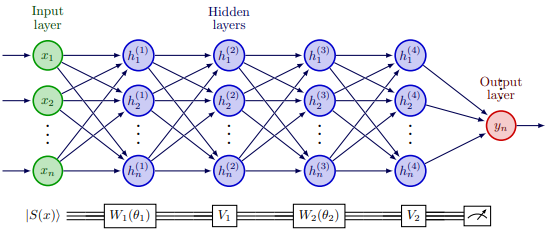
\includegraphics[width=\linewidth]{img/img-ch3/QNN_parallelism.png}
   \caption{Parallelism of a variational circuit with a classical neural network}
   \label{fig:QNN-parallelism}
\end{figure}

After all, we have a model and we can construct it theoretically. However, there is a missing ingredient that we haven not given the proper attention. We have mentioned several times about the optimizable parameter $\theta$, but up to know, we have not done anything about it. Moreover we are in the field of machine learning, so the step that we are missing is the training and that is where the optimization of $\theta$ parameter comes into the picture.


\subsection{Training a quantum neural network}
Training a quantum neural network consist on finding the parameters $\theta$ which minimise a data-dependent cost function. Consider a cost function $C(\theta)$ which relies on a model $f_{\theta}$ that depends on parameters $\theta$. The partial derivative of the cost with respect to $\mu \in \theta$ is
\begin{equation}
    \frac{\partial C}{\partial \mu} = \frac{\partial C}{\partial f_{\theta}} \frac{\partial f_{\theta}}{\partial \mu}
\end{equation}

In the training of variational circuits, $\frac{\partial C}{\partial f_{\theta}}$ is a classical computation, so it can be tackled by classical techniques and libraries. The problem comes when computing the partial derivative of $f_{\theta}$, which is the result of a quantum computation, with respect to $\mu \in \theta$ one of its variational parameters.

To unlock the potential of gradient-descent-based optimization strategies it is needed to have access to the gradients of quantum computations. By providing such partial derivatives, quantum computing can fit into hybrid machine learning pipelines without trouble and be trained.

First, we will go through a basic overview.

The model function of the quantum neural network is a scalar-valued function ${f_{\theta}: \mathbb{R}^N \longrightarrow \mathbb{R}}$. The gradient of the model is the vector of partial derivatives with respect to its parameters $\theta=\left\lbrace \theta_1,...,\theta_K\right\rbrace$,
\begin{equation}
    \nabla f_{\theta}= 
     \begin{bmatrix}
    \frac{\partial f_{\theta}}{\partial \theta_1}\\
    \vdots \\
    \frac{\partial f_{\theta}}{\partial \theta_K}\\
    \end{bmatrix}
\end{equation}

There are different approaches to evaluate the gradients of a numerical computation.
\begin{enumerate}
    \item \textbf{Numerical differentiation.} We can always approximate the partial derivative numerically using the finite-differences method. Next we will apply it to a quantum model $f_{\theta}$ that depends on a parameter $\mu \in \theta$:
    $$\frac{\partial f_{\theta}}{\partial \mu} \approx \frac{f_{\theta} - f_{\theta + \delta \theta}}{|| \delta \theta ||}$$
    where $\delta \theta$ is the parameter set in which $\mu$ has been exchanged by $\mu + \delta \mu$, with $\delta \mu$ an infinitesimal shift.
    
    This is a linear approximation of the model between two different points. In a context where each function evaluation can only be estimated with an error, the finite-difference method is problematic. For small partial derivatives, we need more precision for each function evaluation, so we need more shots to estimate $f_{\theta}$, in other words, more repetitions of the algorithm. In situations when the minimum has to be approximated closely, the optimisation landscape has many saddle points and there is a high variance of the measurements, numerical finite-differences methods are not really suitable. 

    \item \textbf{Automatic differentiation. } It is a programming paradigm in which the gradient is efficiently computed through the accumulation of intermediate derivatives, following the chain rule. A well known automatic differentiation technique is the backpropagation algorithm for the training of classical neural networks.
    
    Unfortunately, for $f_\theta$ it is not clear how this intermediate derivatives could be stored and reused inside of a quantum computation, since the intermediate quantum states cannot be measured without impacting the overall computation and backpropagated information cannot be shared because of the quantum no-cloning theorem.

    \item \textbf{Parameter shift rule.} It comes from the idea of computing a partial derivative of a quantum computation using quantum computation, this means using the same circuit in the quantum neural network, yet shifting the values of the optimizable parameters. To compute gradients of quantum expectation values with respect to one of the variational parameters, the paramether shift rule follows this strategy: first we derive an equation for $\frac{\partial f_{\theta}}{\partial \mu},\, \mu \in \theta$ as a linear combination of the same expectation but with the parameter ``shifted''. The parts of this equation can be evaluated on a quantum computer and consequently combined on a classical coprocessor. Like this, evaluating $\frac{\partial f_{\theta}}{\partial \mu}$ can often be done on a circuit architecture similar or identical to the one of $f_{\theta}$ and requires the  evaluation of the model a few times, generally two, at different points in the parameter space.

    \begin{definicion} [Parameter shift rule]
        Let $f_\mu = \braket{\mathcal{M}}_{\mu}$ be a quantum expectation value that depends on $\mu$ a classical parameter. A parameter shift rule is an identity of the form
        \begin{equation}
            \frac{\partial f_{\mu}}{\partial \mu} = \sum_{i} a_i f_{\mu + s_i}
        \end{equation}
        where $a_i, s_i \in \mathbb{R}$
    \end{definicion}

    A consideration is that the shifts $s_i$ are not necessarily small infinitesimal values. With this computation, the gradient is not approximated, it is exact, however in practice, a quantum computer can only estimate an expectation value and therefore the parameter shift rule lets us compute an estimation of the analytic gradient. In contrast with the finite difference method through which we can compute an estimation of the approximate gradient. 

    There would be no problem with chaining parameter shift rules to compute higher order derivatives such as the Hessian. 
    
\end{enumerate}

To conclude, on one hand we have found a valid method, the parameter shift method, to compute the partial derivatives of quantum computations, thus we can calculate $\frac{\partial f_{\theta}}{\partial \mu}$. On the other hand, $\frac{\partial C}{\partial f_{\theta}}$ is a classical computation, that can be tackled by classical techniques and libraries such as automatic differentiation. In consequence, we can compute the partial derivative of the cost with respect to $\mu \in \theta$, 
\begin{equation}
    \frac{\partial C}{\partial \mu} = \frac{\partial C}{\partial f_{\theta}} \frac{\partial f_{\theta}}{\partial \mu}
\end{equation}
And we are in conditions to be able to apply gradient-descent-based optimization strategies to train quantum neural networks.

So, we have seen how to build a quantum neural network, its structure and operations and then we have figured out how to train it. Everything is proceeding smoothly up to this point. However, quantum neural networks also pose some challenges when it comes to training them that we haven't come accross yet. It is concerning the situations in which the training gradients vanish, and thus, the training can no longer progress. This situation is known as \textbf{Barren plateaus}. 

A vanishing gradient means that with high probability the partial derivatives are close to zero in all their elements, Barren plateaus can be understood as areas in the landscape of the cost function in which the gradients become zero. In turn, the optimisation cannot proceed because the optimisation is slow and expensive. To resolve the small signal and avoid a random walk, high-precision measurements are needed, which are a problem when we are working with noisy near-term quantum computers.

There are different root causes for this phenomenon. They are observed when variational circuit architectures are highly expressive and Hilbert spaces large. To have an idea of what this means we can imagine we are moving over long distances in a very large space, the impact of an individual step towards the ultimate destination does not have a huge effect. Therefore, this derives into an important design principle of variational quantum models: to find a suitable, limited structure for the variational form which restricts training to the relevant subspace of the enormous Hilbert space.

The presence of barren plateaus has a stochastic nature, the high probability of the partial derivatives being zero derives from the statistical properties of partial derivatives. 


\subsection{Considerations on QNN's}

As a conclusion for this section, we will reflect on a series of ideas and concerns to take into consideration regarding quantum neural networks.

\begin{enumerate}
    \item A quantum neural network depends on a feature map, a variational form and a measurement operation. These are three choices we have to make when designing a variational circuit depending on the problem and the data we are dealing with. 

    \item The data is a really important part of any machine learning method. It is what feeds the quantum neural network. We should consider pre-processing techniques according to the nature of the data and the chosen feature map.

    \item The design of the variational form and the number of optimizable parameters it works with is a determining factor for the power of the quantum neural network. If the variational form uses too many parameters, we risk overfitting, while with very few parameters, we would be threatened by underfitting.
    
\end{enumerate}

\nocite{*}

\endinput
%--------------------------------------------------------------------
% FIN DEL CAPÍTULO. 
%--------------------------------------------------------------------
